Below is a figure showing the \textbf{empirical pseudo-regret} of two UCB algorithms: ``original UCB'' (red) vs. ``modified UCB'' (blue), for three different gap values \( \Delta = 0.25, 0.125, \) and \( 0.0625 \). Each curve is the average over 20 runs of length \( T=100000 \), with shaded \( \pm1 \) standard-deviation bands.

\begin{figure}[h]
    \centering
    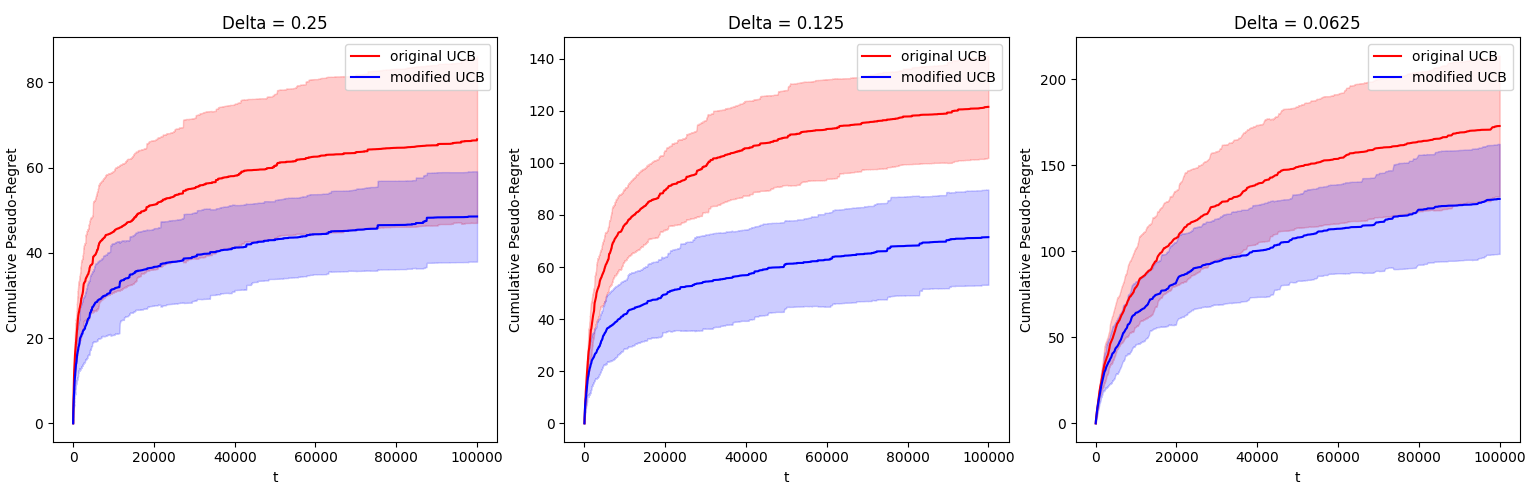
\includegraphics[width=\textwidth]{plots.png}
    \caption{Empirical pseudo-regret over time for different values of \( \Delta \).}
\end{figure}

\subsection{Plot Description}

\begin{itemize}
    \item \textbf{Horizontal axis}: time \( t\in\{1,\dots,100000\} \).
    \item \textbf{Vertical axis}: cumulative pseudo-regret \( \widehat{R}_t \), i.e. \( \sum_{s=1}^t\Delta(A_s) \), where \( \Delta(A_s) \) is the gap between the chosen arm’s mean and the optimal arm’s mean at time \( s \).
    \item \textbf{Subplots}: from left to right, we show the same experiment but with \( \Delta=0.25,\ 0.125,\ \text{and}\ 0.0625 \).
\end{itemize}

In all three cases, the \textbf{blue (modified UCB)} curve remains below the \textbf{red (original UCB)} curve, indicating the modified parametrization typically achieves lower pseudo-regret. We also see that for smaller \( \Delta \) (rightmost plot), overall regret magnitudes are higher.

\subsection{1) Which values of \( \Delta \) lead to higher regret?}

We see from the three subplots that:
\begin{itemize}
    \item \( \Delta=0.25 \) (left) yields smaller final regrets, on the order of \( \approx 80 \) for the original UCB and \( \approx 50 \) for the modified UCB by \( t=100000 \).
    \item \( \Delta=0.125 \) (middle) has higher final regret (\( \approx 140 \) vs. \( \approx 100 \)).
    \item \( \Delta=0.0625 \) (right) yields still higher regrets (\( \approx 220 \) vs. \( \approx 160 \)).
\end{itemize}

Hence, \textbf{the smaller \( \Delta \) is, the higher the pseudo-regret} tends to be. Intuitively, when the arms’ means are closer together, it is harder to distinguish the optimal arm from the suboptimal arm; more exploration is needed before we can reliably exploit.

\subsection{2) Relative performance of the two parametrizations}

Throughout the plots, the \textbf{modified UCB} (“blue”) systematically attains lower pseudo-regret than the “original UCB” (“red”), and the gap between them grows larger over time. This is consistent with the theoretical claim that using a \( \sqrt{\ln t} \) (rather than \( \sqrt{\ln t^3} \) or similar) confidence term can remove an unnecessary union-bound factor, thereby tightening the exploration bonus and improving performance. In short:

\begin{itemize}
    \item \textbf{Modified UCB} explores more selectively, resulting in \textbf{lower regret} in practice.
    \item \textbf{Original UCB} maintains a bigger confidence-radius term and thus “over-explores” somewhat, leading to a higher cumulative regret curve.
\end{itemize}

Hence, \textbf{the modified parametrization outperforms the original} for all three gap values, especially noticeable when the gap is small.